\subsection{Batch Rendering} % (fold)
\label{sub:Batch Rendering}

\subsubsection{研究背景}

傳統上 OpenGL 要畫圖形到螢幕上時,會建立 VAO(Vertex Array Object)用來儲存 VBO (Vertex Buffer Object) 和 IBO (Index Buffer Object),
其中 VBO 儲存圖形的點座標、IBO 儲存 index 座標,最後用 glDrawElements() 讓 OpenGL 將圖形經過 Rendering Pipeline 畫在 Target 上(通常是螢幕或是 Framebuffer)。

\begin{lstlisting}
InitializeRenderer();

for( /* 場景的所有物體 */ )
{
    Render();
}
\end{lstlisting}

但是遊戲引擎在畫場景中的每個物體時,如果每個物體都要重新建構 VBO 和 IBO 時,則會耗費大量時間在從 CPU 傳輸資料到 GPU 中,同時也必須減少 OpenGL 的 State 變換,
因此將渲染前先將多種圖形的頂點收集起來,再一次進行繪製,減少 Draw Call 進而增加可以繪製的圖形數量。

\begin{lstlisting}
InitializeRenderer();
size_t vertex_count = 0;

while( /* 場景還有物體尚未渲染 */ )
{
    CollectVertices();
    vertex_count += size;
    // 超過單次 Draw Call 的上限,先渲染
    if(vertex_count > MAX_VERTEX_COUNT_PER_DRAWCALL)
    {
        Render();
        ResetRenderer();
        vertex_count = 0;
    }
}
\end{lstlisting}

\subsubsection{實作}

以畫矩形作為例子,首先要有辦法操作頂點,因此要有頂點的 class

\begin{lstlisting}
struct QuadVertex
{
    vec3 position;
    vec4 color;
    vec2 texCoord;
    float texIndex;
};
\end{lstlisting}

四個頂點構成一個矩形,所以接著宣告矩形的 class,重載小於運算子是為了要能排序,這在要開啟深度測試時很重要。 \footnote{TODO}

\begin{lstlisting}
struct QuadShape
{
    QuadVertex p[4];

    friend bool operator<(const QuadShape &lhs, const QuadShape &rhs)
    {
        return lhs.p[0].position.z < rhs.p[0].position.z;
    }
};
\end{lstlisting}

接著可以開始著手進行 Renderer 的撰寫:

\begin{lstlisting}
struct QuadRenderer
{
    void init()
    {
        vao = CreateVertexArray();
        
        VBO *vbo = CreateVertexBuffer(MaxQuadVertexCount * sizeof(QuadVertex));
        vbo->SetVertexBufferLayout();
        vao->SetVertexBuffer(vbo);
        
        IBO *ibo = CreateIndexBuffer(MaxQuadIndexCount);
        ibo->SetIndexBuffer( /* 根據 premitive type 的不同 */ );
        vao->SetIndexBuffer(ibo);
        
        // 載入 Shader
        shader = LoadShader();
        shader->initTextureSlots();
    }
    
    void submit(const vec4 position[4], const vec4 &color, const vec2 texCoords[4], float texIndex)
    {
        QuadShape submitQuad{};
        // Add vertices of a quad to buffer
        for(int i = 0; i < 4; i++)
        {
            submitQuad.p[i].position  = position[i];
            submitQuad.p[i].color     = color;
            submitQuad.p[i].texCoord  = texCoords[i];
            submitQuad.p[i].texIndex  = texIndex;
        }
        //
        quadIndexCount += 6;
        //
        quadShapeList.push_back(submitQuad);
    }
    
    void draw(bool DepthTest, const mat4 &ViewProjMatrix)
    {
        if(DepthTest)
            sort(quadShapeList.begin(), quadShapeList.end());
            
        // 設定頂點資料
        vao->setVertexBufferData(quadShapeList);
        
        // 設定 Shader uniform
        shader->setUniformMat4("u_ViewProjection", ViewProjMatrix);
        
        // 渲染
        DrawElement(vao);
    }
    
    VAO *vao = nullptr;
    Shader *shader = nullptr;
    std::vector<QuadShape> quadShapeList;
    uint32_t quadIndexCount = 0;
};
\end{lstlisting}

init() 負責初始化 Renderer 的狀態以及準備 VBO, IBO 和 Shader 的初始化,Renderer 初始化結束後,
便可以開始提交頂點到 Renderer 上,submit() 可以提交要畫的頂點,接著 draw() 在每個 Batch 的最後將頂點渲染,結束這一次的渲染。

\subsubsection{結論}

加入 Batch Rendering 後,RishEngine 的 Renderer 獲得了顯著的提升:

\begin{table}[h]
\centering
    \begin{tabular}{@{} *{5}{c} @{}}
    \headercell{Number of \\ Sprites} & \multicolumn{4}{c@{}}{Modes}\\
    \cmidrule(l){2-5}
    & Debug Non-batch & Release Non-batch & Debug Batch & Release Batch    \\ 
    \midrule
    100    & 1000 &  1055   &  1900 &  2789 \\
    1000   & 167  &  158    &  568  &  1379 \\
    10000  & 18   &  17     &  82   &  247  \\
    100000 & < 1    &  < 1  &  9    &  28   \\
    \end{tabular}
\caption{不同 Rendering 方法下 FPS 差別}
\label{tab:abc}
\end{table}

% 說明文字說明文字說明文字說明文字說明文字說明文字

\begin{figure}[h]
    \begin{subfigure}{0.5\textwidth}
        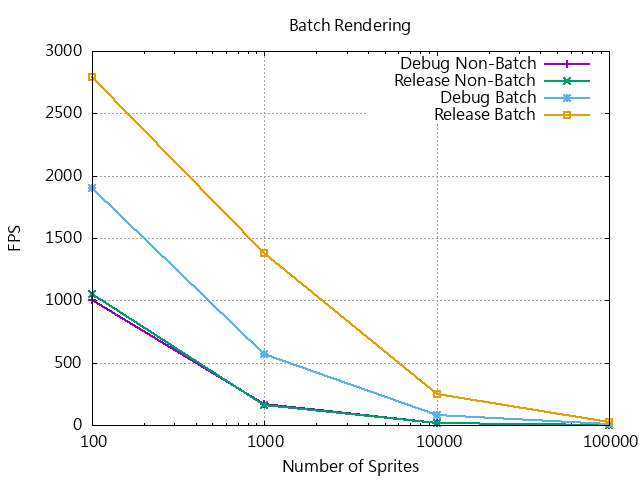
\includegraphics[width=0.9\linewidth, height=5cm]{./resources/batch_compare.png} 
        \caption{不同 Rendering 方法}
        \label{fig:subim1}
    \end{subfigure}
    \begin{subfigure}{0.5\textwidth}
        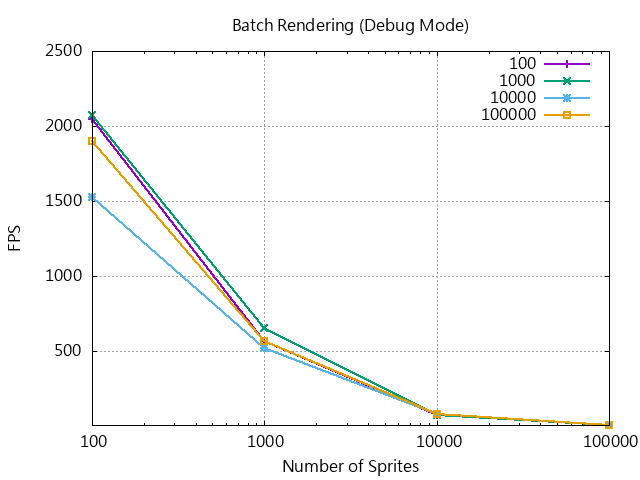
\includegraphics[width=0.9\linewidth, height=5cm]{./resources/max_index.png}
        \caption{不同 Max Index}
        \label{fig:subim2}
    \end{subfigure}
\caption{不同 Rendering 方法效能比較}
\label{fig:image2}
\end{figure}

% 說明文字說明文字說明文字說明文字說明文字說明文字說明文字

\subsubsection{未來展望}

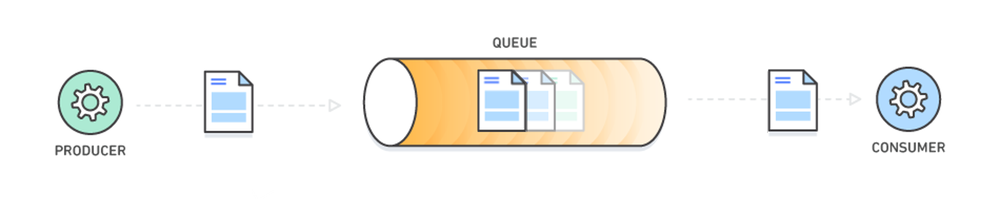
\includegraphics[width=\textwidth]{./resources/cc.png} 

\begin{itemize}
    \item{將 Renderer 變成 Multi-thread 架構}
        \SubItem{由於 OpenGL 在設計當初並沒有考慮到多線程,因此如果要在 OpenGL 使用多線程架構則要用 C++ 模擬,相較於其他現代的 API ,就沒有此限制(Vulkan, DirectX)。}
        \SubItem{將程式分成 Main Thread 與 Rendering Thread}
            \SubSubItem{Main Thread 主要負責遊戲循環,如果要畫東西時,會將 Render 資訊打包成一個 Task,接著加到共用的 Rendering Queue 中(Message Queue)。}
            \SubSubItem{Rendering Thread 負責消化 Rendering Queue 中的 Task ,向 GPU 發起 Draw Call。}
        \SubItem{在原本單線程的 Renderer 中,主要的瓶頸在 Submit Draw Call,繪製時必須等待繪製好了(Blocking),改成多線程則可以解決這個問題。}
\end{itemize}

\newpage
